\chapter{Mass fit to \decay{\Bp}{\Dsp\phiz} candidates} 
\label{ch:B2DsPhi}

\minitoc

In this chapter the methodology used to search for \decay{\Bp}{\Dsp\phiz} decays is described.

{\color{Red}
\begin{itemize}
\item Details of blinding procedure for historic context
\end{itemize}
}

\section{Fit components}
\label{sec:B2DsPhi_fitcomponents}


\subsection{Signal decays}
\label{sec:B2DsPhi_signalcomps}

{\color{Red}
\begin{itemize}
\item plots of signal shapes
\end{itemize}
}


\subsection{Partially reconstructed backgrounds}
\label{sec:B2DsPhi_partrecocomps}


{\color{Red}
\begin{itemize}
\item plots of partreco shapes
\end{itemize}
}

\subsection{Combinatorial  backgrounds}
\label{sec:B2DsPhi_combcomps}



\section{Fit strategy}
\label{sec:B2DsPhi_fitstrategy}

The yield of \decay{\Bp}{\Dsp\phiz} candidates are determined using a simultaneous unbinned maximum likelihood fit in a number of different categories.
These categories are designed to help separate the different contributions such that the relative contributions can be distinguished.




\subsection{Simultaneous categories}
\label{sec:B2DsPhi_fitstrategy}

{\color{Red}
\begin{itemize}
\item \Dsp decay mode categories
\item $m(\Kp\Km)$ invariant mass categories 
\item helicity angle categories 
\item MC plots of each
\end{itemize}
}

\subsection{\decay{\Bp}{\Dsp \Kp \Km} model assumptions}
\label{sec:B2DsPhi_B2DsKKModel}

{\color{Red}
\begin{itemize}
\item Studies with Laura++
\item distributions of a number of models
\item refer to \Dsp\Kp\Km plot
\item final fraction
\end{itemize}
}

\subsection{Fit validation}
\label{sec:B2DsPhi_fitstrategy}

{\color{Red}
\begin{itemize}
\item Toy distributions
\end{itemize}
}

\section{Normalisation and signal fits}




%%%%%%%%%%%%%%%%%%%%%%%%%%%%%%%%%%%%%%%%%%%%%%%%%%%%%%%%%%
\begin{figure}[!h]
    \centering
    \begin{subfigure}[t]{1.0\textwidth}
        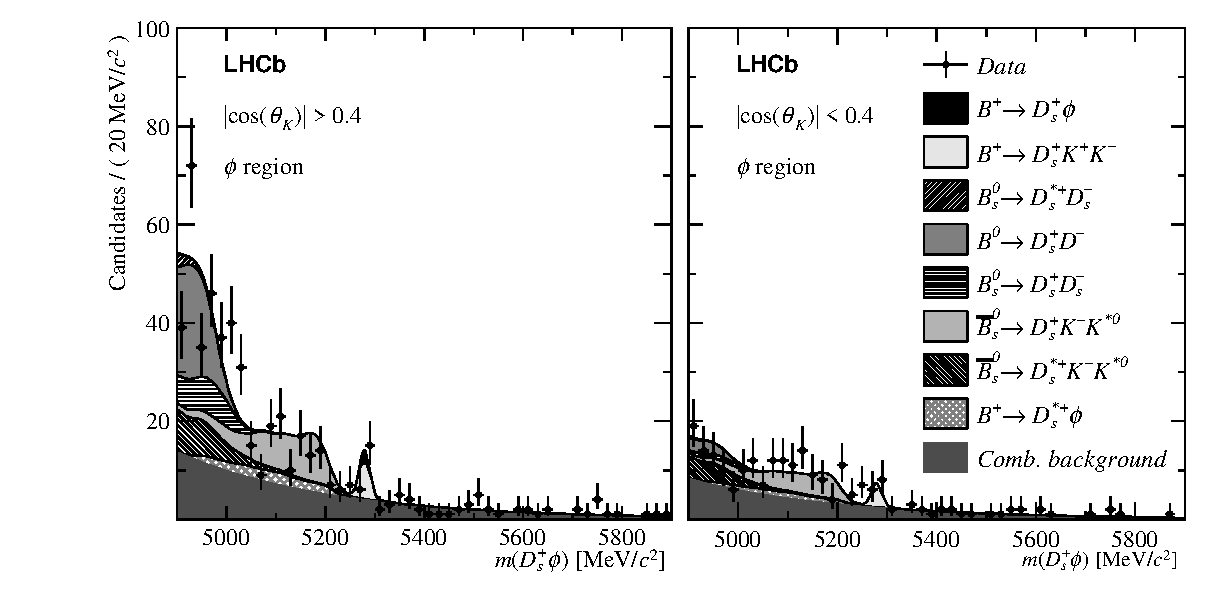
\includegraphics[width=1.0\textwidth]{figs/B2DsPhi/Fig4a.eps}
        %\caption{Normalisation without selection}
    \end{subfigure}
    \begin{subfigure}[t]{1.0\textwidth}
        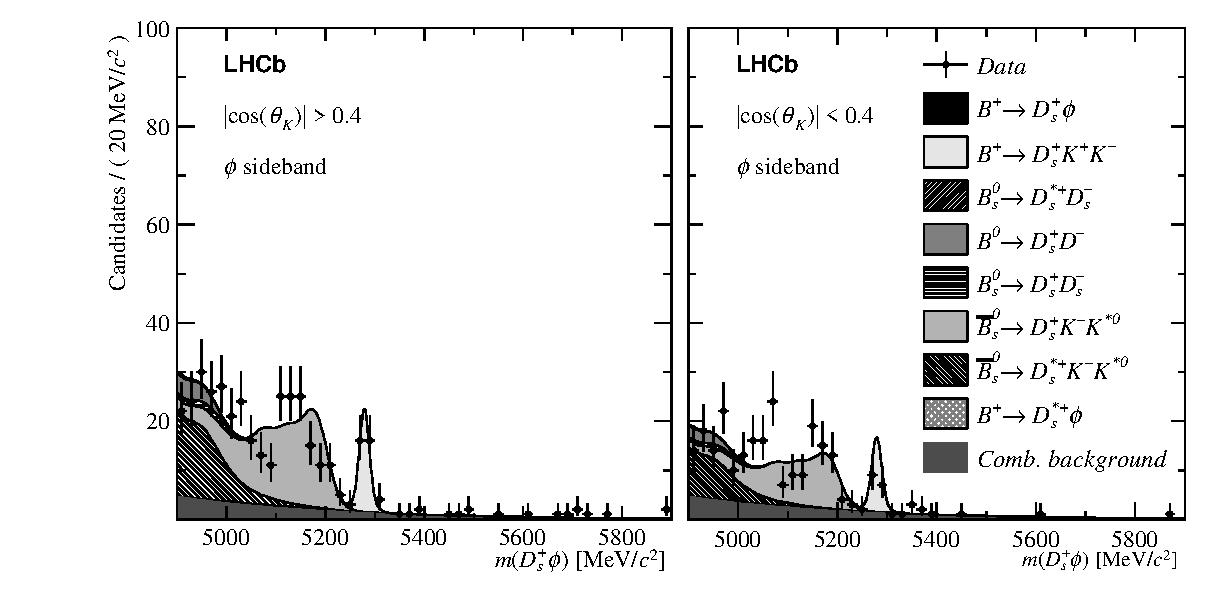
\includegraphics[width=1.0\textwidth]{figs/B2DsPhi/Fig4b.eps}
        %\caption{Normalisation without selection}
    \end{subfigure}
    \caption{Invariant mass fits to \decay{\Bp}{\Dsp\Kp\Km} candidates}
\end{figure}
%%%%%%%%%%%%%%%%%%%%%%%%%%%%%%%%%%%%%%%%%%%%%%%%%%%%%%%%%%


\section{Efficiency corrections}
\label{sec:B2DsPhi_effcorrections}


{\color{Red}
\begin{itemize}
\item Assume pseudo two body decay, therefore simple ratio  
\end{itemize}
}

\section{Systematic uncertainties}
\label{sec:B2DsPhi_systuncertainy}



\section{Results}
\label{sec:B2DsPhi_results}

{\color{Red}
\begin{itemize}
\item Copy most of results section from paper
\end{itemize}
}




\subsection{Limit setting}
\label{sec:B2DsPhi_limitsetting}

{\color{Red}
\begin{itemize}
\item Document all methods attemped
\item CLs plots
\item likelihood
\item FC bands
\item Table of comparison 
\end{itemize}
}

%%%%%%%%%%%%%%%%%%%%%%%%%%%%%%%%%%%%%%%%%%%%%%%%%%%%%%%%%%
\begin{figure}[!h]
    \centering
        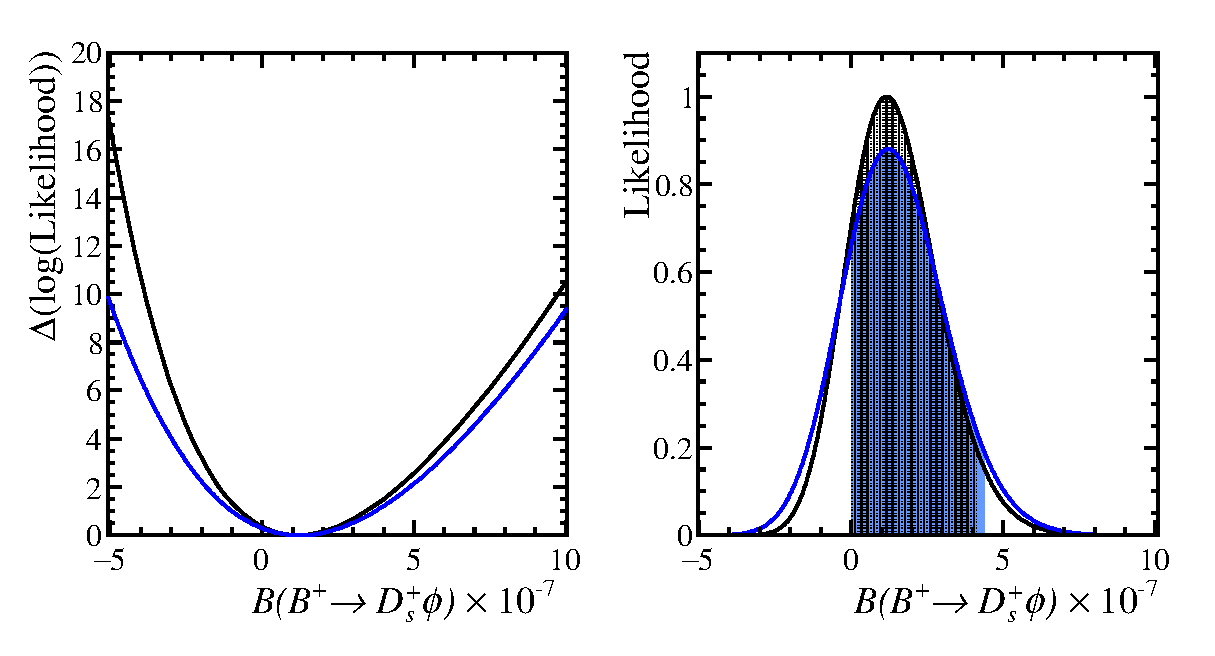
\includegraphics[width=1.0\textwidth]{figs/B2DsPhi/Likelihood_limits.eps}
        \caption{Bayesian profile likelihood limit determination}
    \label{fig:limit_likelihood}   
\end{figure}
%%%%%%%%%%%%%%%%%%%%%%%%%%%%%%%%%%%%%%%%%%%%%%%%%%%%%%%%%%

%%%%%%%%%%%%%%%%%%%%%%%%%%%%%%%%%%%%%%%%%%%%%%%%%%%%%%%%%%
\begin{figure}[!h]
    \centering
        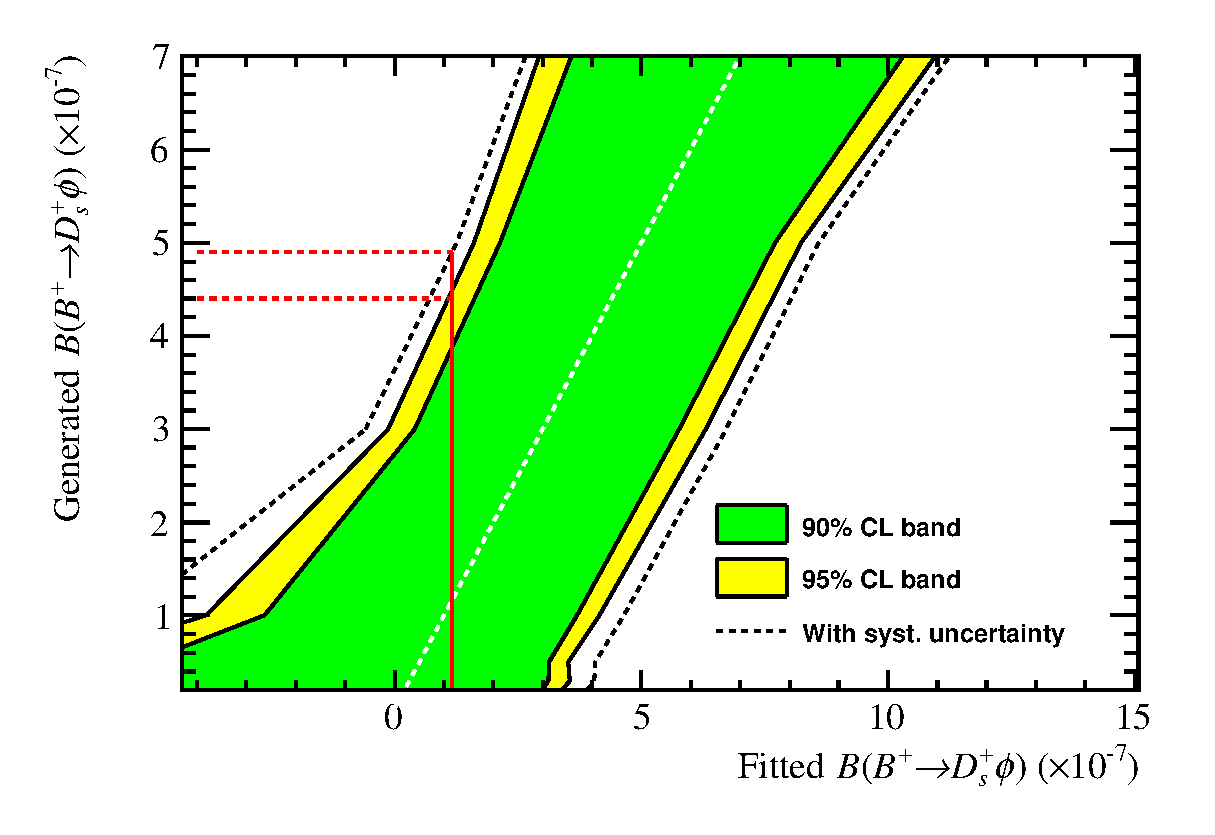
\includegraphics[width=0.8\textwidth]{figs/B2DsPhi/Sensitivity_plot.eps}
        \caption{CLs limit determination}
    \label{fig:limit_cls}   
\end{figure}
%%%%%%%%%%%%%%%%%%%%%%%%%%%%%%%%%%%%%%%%%%%%%%%%%%%%%%%%%%

